\chapter{狭义相对论}
\section{4维表述基础}
\subsection{预备知识}
不论是否发生了什么,空间的一点和时间的一瞬的结合就叫一个\textcolor{blue}{事件}(event).全部事件的集合叫\textcolor{blue}{时空}(spacetime).狭义相对论中谈及的\textcolor{blue}{粒子}(particle)是模型化语言,是完全没有大小的点,分为有静质量的粒子(质点)和无静质量的粒子(光子,photon)两类.一个粒子的全部历史由一系列事件组成,因此对应于时空中的一条曲线,称为该粒子的\textcolor{blue}{世界线}(world line),如图\ref{fig:6-1}所示.
\begin{figure}[htbp]
    \centering
 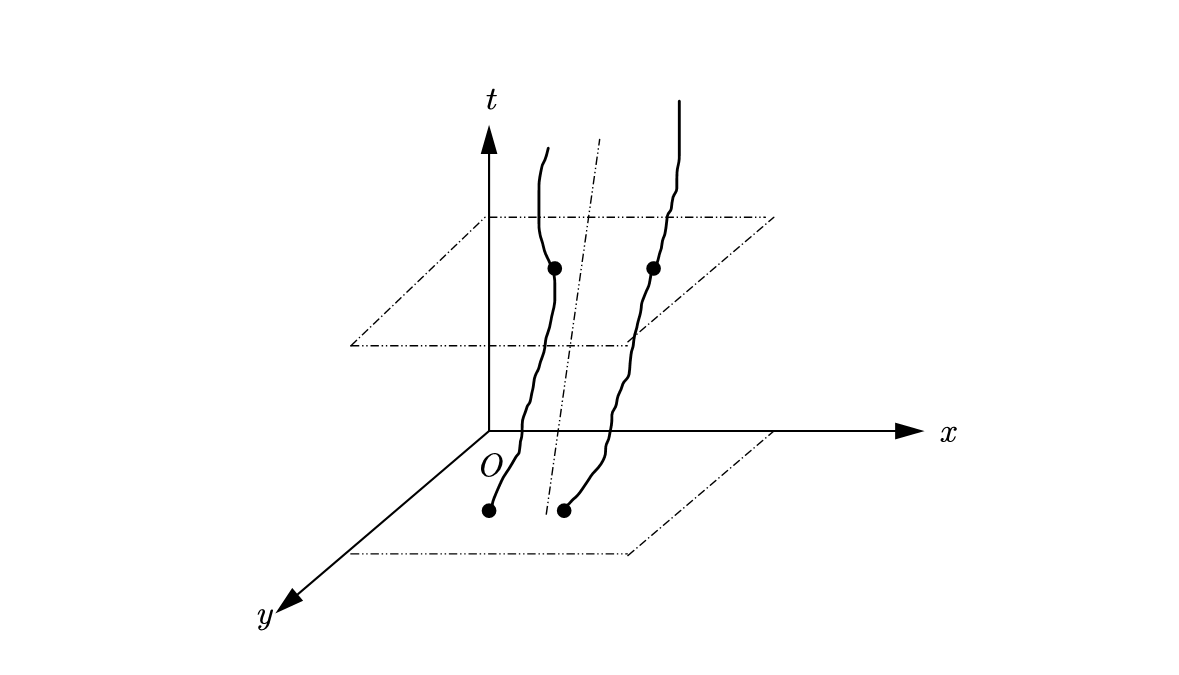
\includegraphics[width=0.8\textwidth]{Pictures/6-1.png}
    \caption{世界线}
    \label{fig:6-1}
\end{figure}

进行物理观测的人叫观察者,将之模型化看成质点,简称\textcolor{blue}{观者}.为了观测,观者手中应有一个走时准确的钟,叫\textcolor{blue}{标准钟}(standard clock),该钟的读数称为该观者的\textcolor{blue}{固有时}(proper time).固有时$\tau$无非是质点世界线的一个特殊参数.
无数观者的集合$\mathscr{R}$叫一个\textcolor{blue}{参考系}(reference frame),满足时空或其一个开子集中的任一点有且仅有$\mathscr{R}$内的一个观者的世界线经过.参考系即世界线的线汇,即对于参考系
\begin{itemize}
\item 过任意事件均有一条世界线.
\item 世界线不相交.
\end{itemize}

\begin{figure}[htbp]
    \centering
 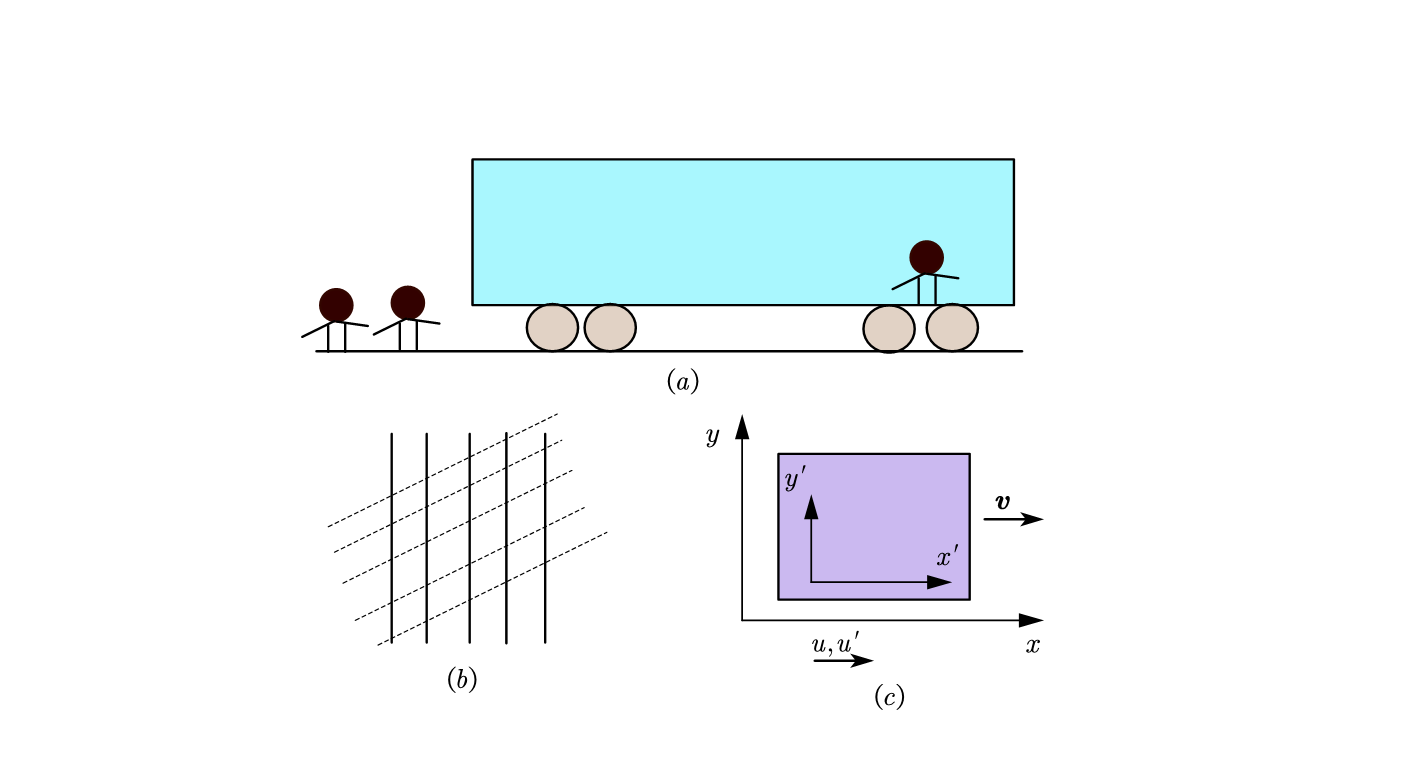
\includegraphics[width=1.2\textwidth]{Pictures/6-2.png}
    \caption{(a):地面系和火车系示意图;(b):地面系(实线)和火车系(虚线)的世界线;(c):Galileo变换}
    \label{fig:6-2}
\end{figure}

如上图\ref{fig:6-2}所示,(a)代表火车系和地面系,而(b)中以许多竖直实线代表地面系观者们的世界线,火车系观者们的世界线则是许多互相平行的斜直虚线.(c)表示Galileo变换,与Galileo相对性原理(任两个惯性系都是平权的)构成Galileo的两大理论贡献.如(c)所示,Galileo变换的坐标变换公式为:
\begin{align}
    \left\{
    \begin{aligned}
        x^\prime&=x-vt\\
        y^\prime&=y\\
        z^\prime&=z\\
        t^\prime&=t
    \end{aligned}
    \right.
\end{align}
坐标变换公式中最后一式蕴含了同时性的绝对性.速度合成公式为:
\begin{align}
    \boldsymbol{u}^\prime=\boldsymbol{u}-\boldsymbol{v}.
\end{align}
\subsection{Maxwell方程的参考系问题}
Maxwell方程组表明Galileo相对性原理对于电磁理论并不成立.于是存在以下两种非此即彼的选择:
\begin{itemize}
\item 认为相对性原理并不总是成立的,即惯性系不平权.存在一个特殊的惯性系(以太,ether),其中光速为c,而其他惯性系则不然.
\item 坚持相对性原理总是成立的.
\end{itemize}

\begin{figure}[htbp]
    \centering
 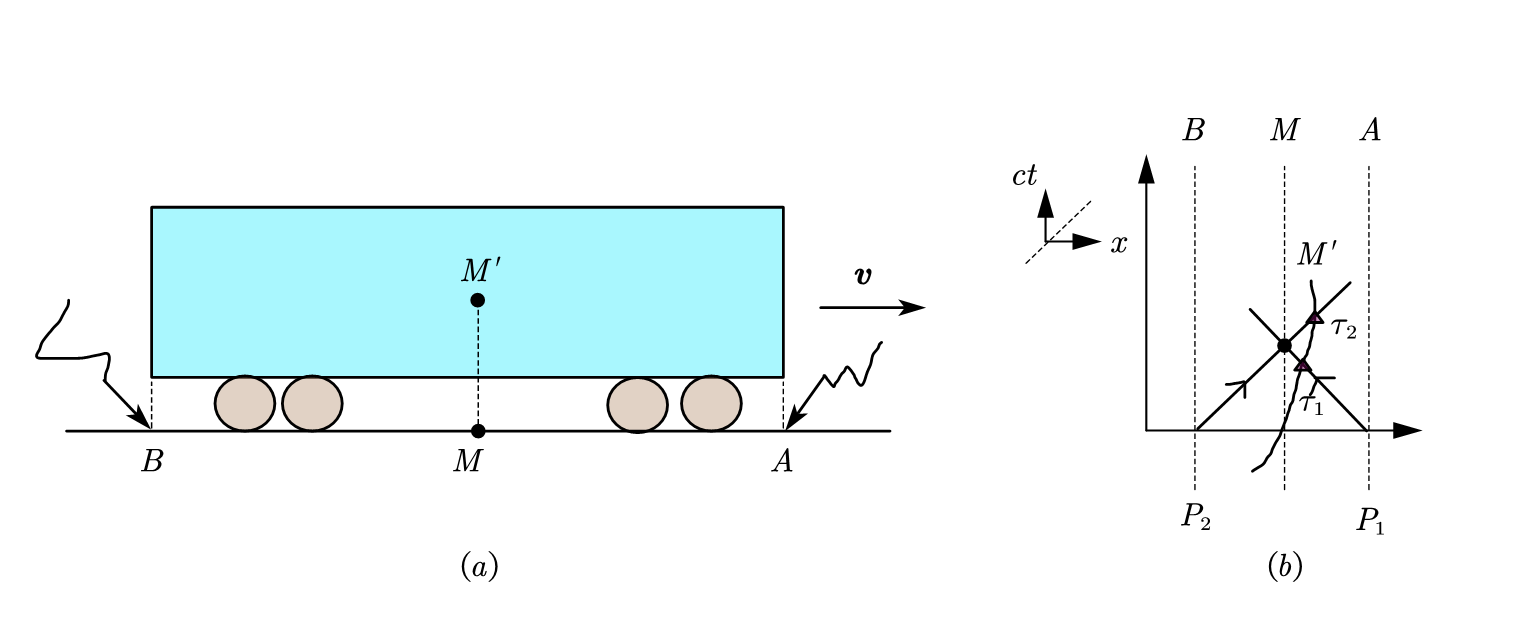
\includegraphics[width=\textwidth]{Pictures/6-3.png}
    \caption{(a):闪电击中车头和车尾;(b):利用世界线进行分析}
    \label{fig:6-3}
\end{figure}

如图\ref{fig:6-3}(a),闪电分别击中火车车头$A$和车尾$B$,地面系$M$认为$A$和$B$同时遭受雷击,而火车系$M^\prime$认为并不同时,车头$A$首先遭受雷击.这表明了“同时的相对性”.以四维语言的时空图分析,地面系$M$的世界线为$P_2P_1$的中垂线,从$P_2,P_1$处发的光自然同时到达$M$.而火车系$M^\prime$的世界线却首先和$P_1$发出的光相遇(时间记为$\tau_1$),其次再和$P_2$相遇(时间记为$\tau_2$),显然$\tau_1<\tau_2$.

狭义相对论的两条假设为:
\begin{itemize}
\item 狭义相对性原理
\item 光速不变性
\end{itemize}
并假设空间是均匀的,各向同性的.

狭义相对性原理包含两个层次的内容:
\begin{itemize}
    \item 在所有观者(质点)中存在一类特殊观者,称为\textcolor{blue}{惯性观者}(inertial observer),与其他观者有绝对区别.在所有观者组成的集合中可以选出一个特殊的子集,其中每个元素都是惯性观者.
    \item 各惯性观者平权,不存在特殊的惯性观者,在由惯性观者组成的子集中不能选出与众不同的元素.
\end{itemize}

洛伦兹变换($v<c$,$c$取为1)为:
\begin{align}
    \left.
\begin{aligned}
    x^\prime&=\gamma(x-vt),\gamma=\dfrac{1}{\sqrt{1-v^2}}\\
    t^\prime&=\gamma(t-vx)
\end{aligned}
\right\}\Rightarrow
\left\{
\begin{aligned}
    u_x^\prime&=\dfrac{u_x-v}{1-u_xv}\\
    u_y^\prime&=\dfrac{u_y}{\gamma(1-u_xv)}\\
    u_z^\prime&=\dfrac{u_z}{\gamma(1-u_xv)}
\end{aligned}
\right.
\end{align}
另一个效果是间隔不变性:
\begin{align}
    \begin{aligned}
        \text{d}I^2&\equiv-\text{d}t^2+\text{d}x^2+\text{d}y^2+\text{d}z^2\\
        \text{d}I^{\prime2}&\equiv-\text{d}t^{\prime2}+\text{d}x^{\prime2}+\text{d}y^{\prime2}+\text{d}z^{\prime2}\\
        \text{d}I^2&=\text{d}I^{\prime2}
    \end{aligned}
\end{align}

\subsection{几何语言重新表述SR}
$$
\begin{aligned}
    \text{牛顿引力论}&\to (\mathbb{R}^4,?)\\
    \text{SR}&\to (\mathbb{R}^4,\eta_{ab})\\
    \text{GR}&\to (\underset{\underset{\text{联通的}}{\downarrow}}{M},g_{ab})
\end{aligned}
\Longrightarrow
\left\{
\begin{aligned}
\overset{\underset{}{\text{物理}}}{\text{惯性系坐标}}&\to \overset{\underset{}{\text{数学}}}{\text{洛伦兹坐标}}\\
\text{间隔不变}&\to \text{线元不变}\\
\text{背景}&\to \text{闵氏时空}\\
\end{aligned}
\right.
$$

\begin{figure}[htbp]
    \centering
 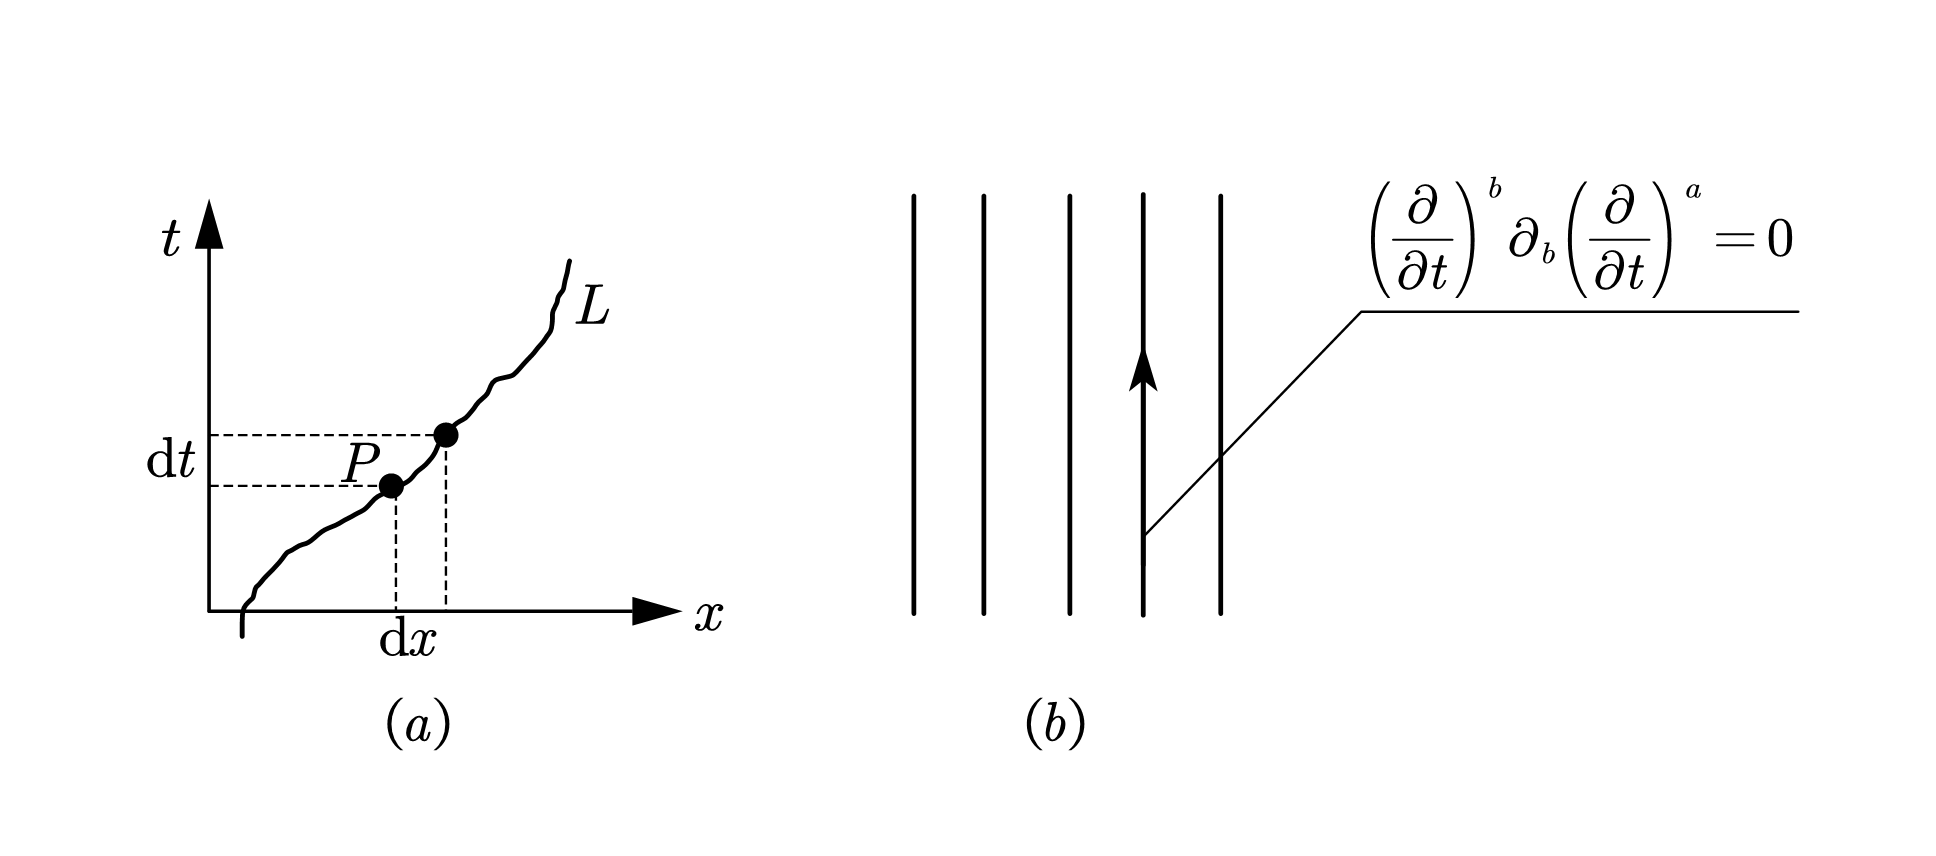
\includegraphics[width=\textwidth]{Pictures/6-4.png}
    \caption{(a):狭义相对论的4维语言表述;(b):任意惯性观者的世界线都是类时测地线}
    \label{fig:6-4}
\end{figure}

如图\ref{fig:6-4}所示,设$L$为粒子的世界线,$p,q$为其上两个邻近的点,粒子在$p$时相对于某惯性系$\mathscr{R}$的速率定义为:
\begin{align}
    u:=\dfrac{\sqrt{\text{d}x^2+\text{d}y^2+\text{d}z^2}}{\text{d}t}
\Longrightarrow
\begin{aligned}
    \text{d}s^2&=-\text{d}t^2+\text{d}x^2+\text{d}y^2+\text{d}z^2\\
    &=-\text{d}t^2\left[-\left(\dfrac{\text{d}x^2}{\text{d}t^2}+\dfrac{\text{d}y^2}{\text{d}t^2}+\dfrac{\text{d}z^2}{\text{d}t^2}\right)\right]\\
    &=-(1-u^2)\text{d}t^2
\end{aligned}
\end{align}
从而
$$
\begin{aligned}
\text{d}s^2&=0\Longleftrightarrow u=1 \Longleftrightarrow null\\
\text{d}s^2&<0\Longleftrightarrow u<1 \Longleftrightarrow timelike  
\end{aligned}
$$

这表明狭义相对论的两个基本信条:“光子相对于任何惯性系的速率$u=1$”和“质点相对于任何惯性系的速率$u<1$”采用4维语言可以改写如下:
\begin{itemize}
    \item 光子世界线是闵氏时空的类光曲线.
    \item 质点世界线是闵氏时空的类时曲线.
\end{itemize}

根据3维语言的狭义相对论,惯性观者相对于所在的惯性坐标系$\{t,x,y,z\}$的速率$u=0$,因而其世界线重合于一条$t$坐标线(如图\ref{fig:6-4}(b)所示).设$\partial_b$是该系的普通导数算符,则有
\begin{align}\label{eq:6.6}
    \partial_b\left(\dfrac{\partial}{\partial t}\right)^a=0\Rightarrow \left(\dfrac{\partial}{\partial t}\right)^b\partial_b\left(\dfrac{\partial}{\partial t}\right)^a=0.
\end{align}

由于物理上的惯性坐标系就是数学上的洛伦兹坐标系,则$\partial_b$就是与闵氏度规$\eta_{ab}$相适配的导数算符,即$\partial_a\eta_{bc}=0$,所以式\ref{eq:6.6}是闵氏时空的测地线方程,可见任意惯性观者的世界线都是类时测地线.反之可证,给定任一类时测地线$G$,总可以找到一个洛伦兹坐标系使得$G$是该系的一条$t$坐标线,因而代表一个惯性观者.从而物理上的惯性观者就对应于数学上的类时测地线,或者说惯性观者的世界线就是类时测地线.

$$
\begin{aligned}
\overset{\boldsymbol{Phys.}}{inertial \ corrdinates} &\longleftrightarrow \overset{\boldsymbol{Math.}}{Lorentizian \ coordinates}\\
\underset{\text{间隔}}{interval}&\longleftrightarrow Minkowski\ line\ element\\
background\ spacetime &\longleftrightarrow 4-dim\ Minkowski \ space\\
observer(point mass) &\longleftrightarrow timelike\ curve\\
\underset{\text{惯性观者}}{inertial\quad observer}&\longleftrightarrow timelike\ geodesic
\end{aligned}
$$

洛伦兹坐标系的每一$t$坐标线都对应于一个惯性观者,该系的全体$t$坐标线组成的参考系称为\textcolor{blue}{惯性参考系},而该坐标系则称为该惯性参考系内的一个\textcolor{blue}{惯性坐标系},不认真区分时,将惯性参考系和惯性坐标系统称为\textcolor{blue}{惯性系},其定义域为全时空(整个$\mathbb{R}^4$),亦称为整体惯性系.属于同一惯性参考系的所有惯性观者的世界线是平行测地线.反之,若两个惯性观者分属不同惯性参考系,则它们的世界线为不平行测地线.一个质点叫做“自由的”或者“做惯性运动的”,若其世界线为测地线.

4维闵氏时空$(\mathbb{R}^4,\eta_{ab})$中洛伦兹系之间的坐标变换对应于$(\mathbb{R}^4,\eta_{ab})$的等度规映射.任一等度规映射可以由若干基本的等度规映射复合而成,后者分为“连续”和“分立”两种.“分立”包括反射和反演,“连续”包括以下三种:
\begin{enumerate}
    \item \textcolor{blue}{平移},由4个独立的Killing矢量场$\left(\dfrac{\partial }{\partial t}\right)^a,\left(\dfrac{\partial }{\partial x}\right)^a,\left(\dfrac{\partial }{\partial y}\right)^a,\left(\dfrac{\partial }{\partial z}\right)^a$表征.
    
    时间平移:
    \begin{align}
    \left\{
    \begin{aligned}
    t^\prime&=t+a\\
    x^\prime&=x\\
    y^\prime&=y\\
    z^\prime&=z
    \end{aligned}
    \right.
    \end{align}
    物理上对应于把惯性系$\mathscr{R}$内所有观者的标准钟的初始设定值增加数值$a$.
    \item \textcolor{blue}{空间转动},由3个独立的Killing矢量场$-y\left(\dfrac{\partial }{\partial x}\right)^a+x\left(\dfrac{\partial }{\partial y}\right)^a,-z\left(\dfrac{\partial }{\partial y}\right)^a+y\left(\dfrac{\partial }{\partial z}\right)^a,-x\left(\dfrac{\partial }{\partial z}\right)^a+z\left(\dfrac{\partial }{\partial x}\right)^a$表征.
    
    $x-y$面内的转动:
    \begin{align}
    \left\{
    \begin{aligned}
    t^\prime &=t\\
    z^\prime &=z\\
    x^\prime&=x\cos\alpha-y\sin\alpha\\
    y^\prime&=x\sin\alpha+y\cos\alpha
    \end{aligned}
    \right.
\end{align}
物理上对应于惯性参考系内部的一个空间坐标变换.
\item \textcolor{blue}{伪转动},由3个独立的Killing矢量场$t\left(\dfrac{\partial }{\partial x}\right)^a+x\left(\dfrac{\partial }{\partial t}\right)^a,t\left(\dfrac{\partial }{\partial y}\right)^a+y\left(\dfrac{\partial }{\partial t}\right)^a,t\left(\dfrac{\partial }{\partial z}\right)^a+z\left(\dfrac{\partial }{\partial t}\right)^a$表征.

$t-x$面内的伪转动:
\begin{align}
\left\{
\begin{aligned}
t^\prime &=\gamma(t-vx)\\
x^\prime&=\gamma(x-vt)\\
y^\prime&=y\\
z^\prime &=z
\end{aligned}
\right.
\end{align}
物理上对应于两个惯性系$\mathscr{R},\mathscr{R}^\prime$之间的坐标变换——洛伦兹变换.
\end{enumerate}

平移和空间转动都是同一惯性参考系内的坐标变换,而伪转动相联系的两个惯性坐标系必然分属两个不同的惯性参考系.

一个钟称为\textcolor{blue}{标准钟}或者\textcolor{blue}{理想钟}(ideal clock),若它在自己世界线上任两点$p_1,p_2$的读数差$\tau_1,\tau_2$之差等于该线在$p_1,p_2$之间的线长,即
\begin{align}
    \tau_2-\tau_1=\int_{p_1}^{p_2}\sqrt{-\text{d}s^2}.
\end{align}
若光速$c$不为1,则上式右边要乘上$\dfrac{1}{c}$.今后谈及世界线时默认以固有时$\tau$为参数,而固有时间等于线长,因此切矢$\left(\dfrac{\partial}{\partial \tau}\right)^a$的长度为1.由于类光曲线线长恒为零,所以光子没有固有时概念,不能充当观者.

标准钟只对\textcolor{blue}{走时率}提出要求,世界线上任意两点的读数差等于线长,而参考系内的钟同步问题则只涉及\textcolor{blue}{初始零点设定}(setting).惯性参考系必须对齐零点,称为\textcolor{blue}{钟同步}(clock synchronization),图\ref{fig:6-5}(b)是用以钟同步的雷达法.
\begin{figure}[htbp]
    \centering
 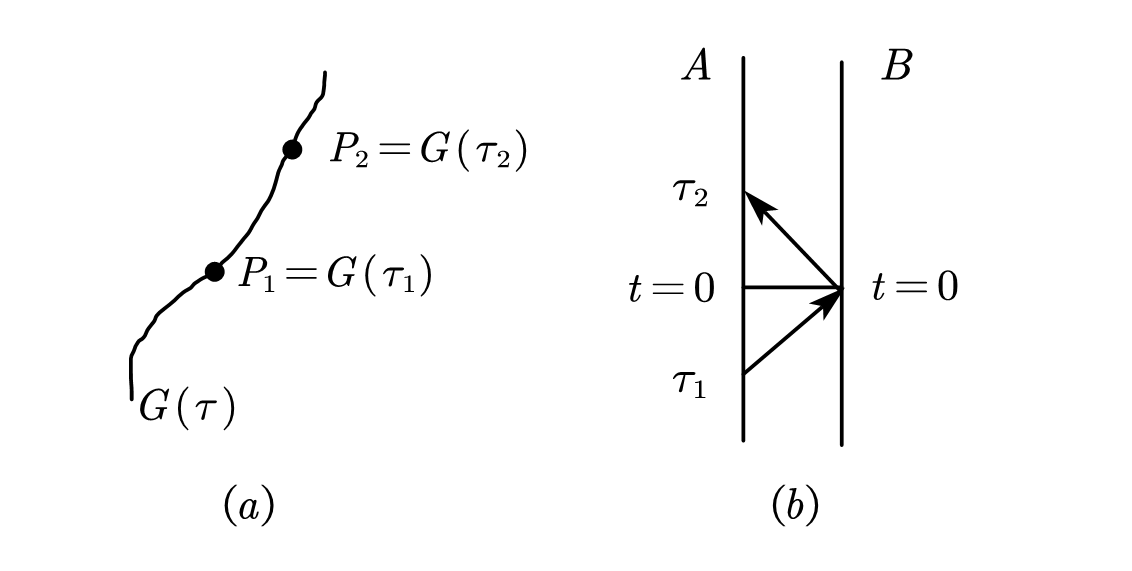
\includegraphics[width=0.8\textwidth]{Pictures/6-5.png}
    \caption{(a):标准钟;(b):钟同步}
    \label{fig:6-5}
\end{figure}

设$x^0$是坐标系的类时坐标,$\eta_{ab}\left(\dfrac{\partial}{\partial x^0}\right)^a\left(\dfrac{\partial}{\partial x^0}\right)^b<0$,$x^1,x^2,x^3$为类空坐标,$\eta_{ab}\left(\dfrac{\partial}{\partial x^0}\right)^a\left(\dfrac{\partial}{\partial x^0}\right)^b>0,i=1,2,3$,则坐标域中任一点$p$的$x^0$值称为事件$p$在该系的\textcolor{blue}{坐标时}(coordinate time).惯性系的坐标时叫做\textcolor{blue}{惯性坐标时},其定义域为全$\mathbb{R}^4$.坐标时与固有时的区别在于:
\begin{itemize}
    \item 固有时只对世界线上的点而言,脱离世界线就没有固有时概念.坐标时与世界线无关,坐标域中的任一点都可谈及它在该系的坐标时.
    \item 同一时空点在不同坐标系中可有不同的坐标时,而固有时与坐标系无关.
\end{itemize}

设$L(\tau)$是某质点的世界线,$\tau$为固有时,$t$为惯性系$\mathscr{R}$的坐标时,则
\begin{align}
    \dfrac{\text{d}t}{\text{d}\tau}= \dfrac{\text{d}t}{\sqrt{-\text{d}s^2}}= \dfrac{\text{d}t}{\sqrt{1-u^2}\text{d}t}=\dfrac{1}{\sqrt{1-u^2}}=\gamma_u,
\end{align}
其中$u$是质点相对于$\mathscr{R}$的速率.

\begin{figure}[htbp]
    \centering
    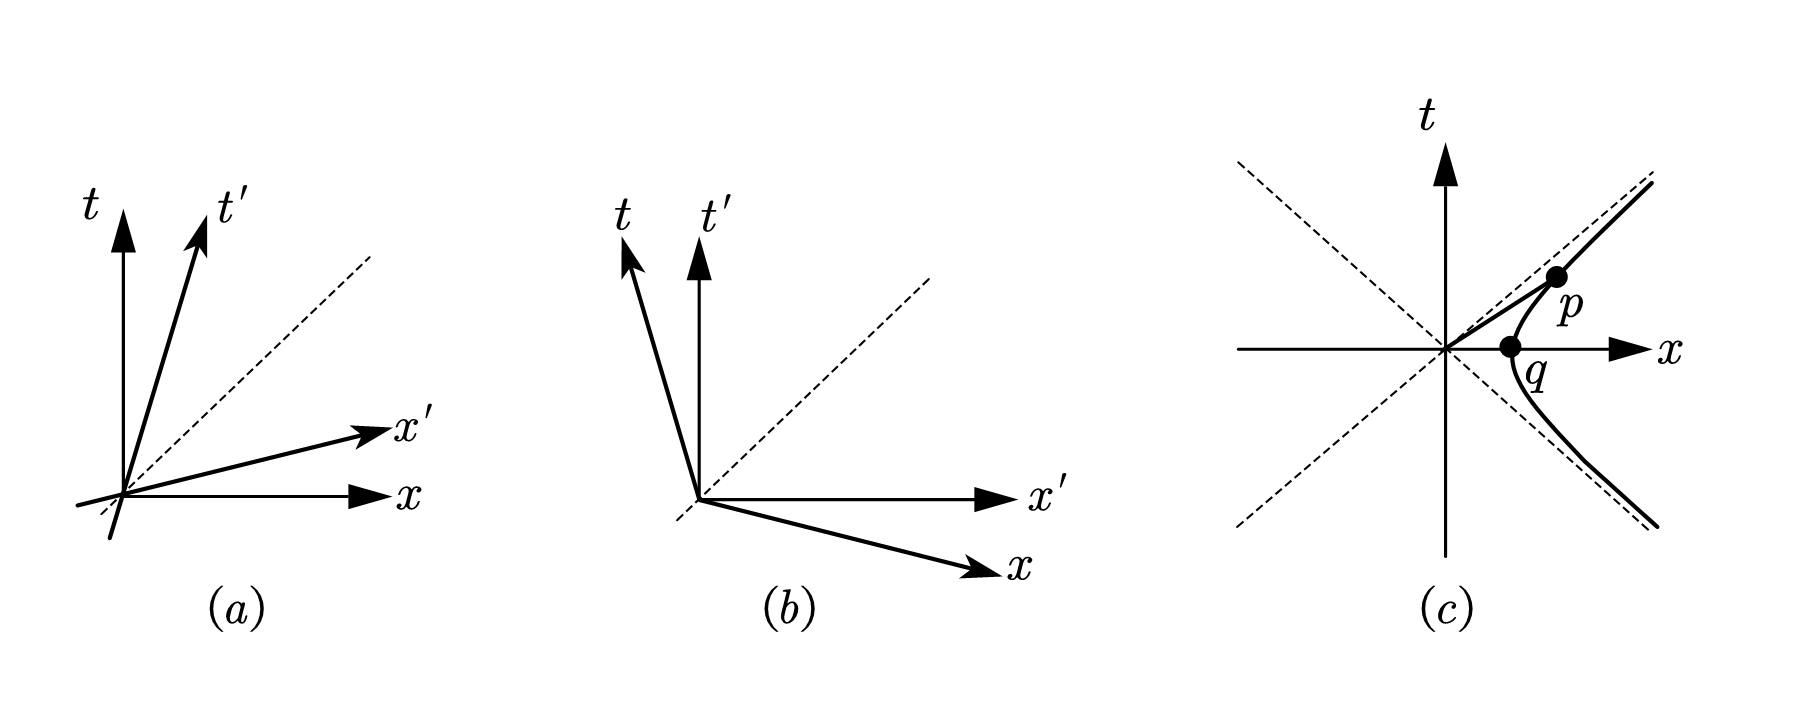
\includegraphics[width=\textwidth]{Pictures/6-6.png}
    \caption{(a): 以$\mathscr{R}$为基准的时空图,$x^\prime$与$t^\prime$分居$45^\circ$线两侧;
    (b): 以$\mathscr{R}^\prime$为基准的时空图,与(a)等价;(c):校准曲线}
    \label{fig:6-6}
\end{figure}

如图\ref{fig:6-6}(a)所示,以惯性系$\mathscr{R}$为基准,将$t^\prime=0,x^\prime=0$分别代入洛伦兹变换,
\begin{align}
\begin{aligned}
    0&=t^\prime=\gamma(t-vx)\Rightarrow t=vx,\\
 0&=x^\prime=\gamma(x-vt)\Rightarrow t=\dfrac{x}{v}.
\end{aligned}
\end{align}
可见,$t^\prime,x^\prime$是过原点,且斜率分别为$\dfrac{1}{v},v$的直线.这两条直线分居虚线两侧且与该线夹角相等.若以以惯性系$\mathscr{R}^\prime$为基准,则时空图如\ref{fig:6-6}(b)所示,注意此时$\left(\dfrac{\partial}{\partial t^\prime}\right)^a,\left(\dfrac{\partial}{\partial x^\prime}\right)^b$以闵氏度规$\eta_{ab}$衡量依旧正交.

设$p=(t.x)$为任一时空点,其与坐标原点之间的直线段的线长按照闵氏度规为$l=\sqrt{|-t^2+x^2|}$.可见双曲线$-t^2+x^2=K(\text{常数})$上面各个点与坐标原点所连接的直线段等长,如图\ref{fig:6-6}(c)所示,称为\textcolor{blue}{校准曲线}.

\subsection{两种时空结构的对比}

相对论中时空是第一手概念,时间与空间则是派生的概念,只有借助参考系把时空进行“3+1”分解才得到时间和空间的概念,同一时空存在着许多不同的3+1分解方案.非相对论物理学默认时空流形是$\mathbb{R}^4$,且具有某些内禀的附加结构,其一就是存在一个称为\textcolor{blue}{绝对时间}(absolute time)的光滑函数$t:\mathbb{R}^4\to\mathbb{R}$,使得$\mathbb{R}^4$被分为无限多层,每层是一个等$t$面$\sum_t$,称为\textcolor{blue}{绝对同时面}(absolute simultaneity surface),它有3维欧式度规,代表$t$时刻的整个三维空间.

给定事件$p\in \mathbb{R}^4$,总有$\mathbb{R}^4-\{p\}=M_1\cup M_2\cup M_3,$其中,
$$
\begin{aligned}
    M_1&\equiv\{q\in M|\text{存在先经历}q\text{后经历}p\text{的观者}\};\\
    M_2&\equiv\{q\in M|\text{存在先经历}p\text{后经历}q\text{的观者}\};\\
    M_3&\equiv\{q\in M|\text{不存在既经历}q\text{又经历}p\text{的观者}\}.
\end{aligned}
$$
\begin{figure}[htbp]
    \centering
    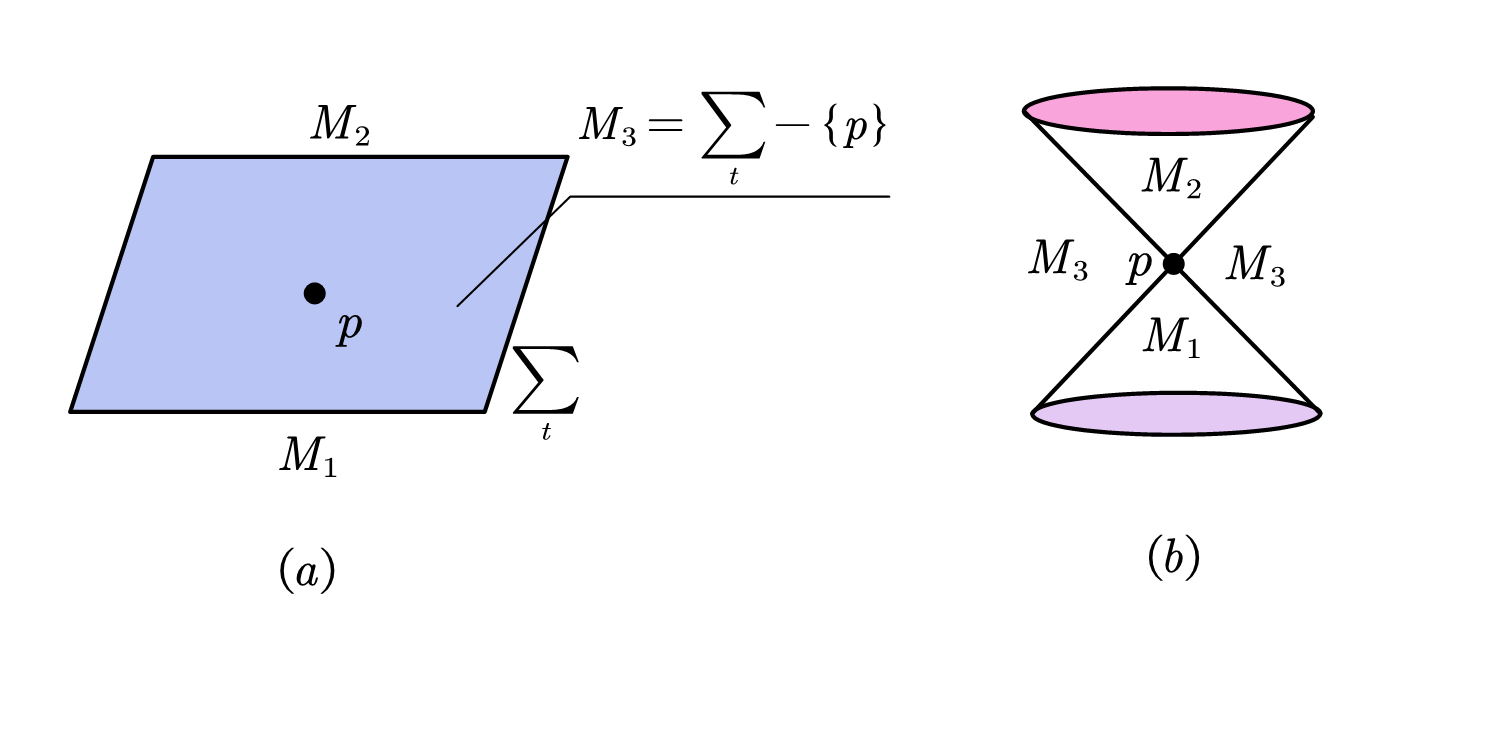
\includegraphics[width=\textwidth]{Pictures/6-7.png}
    \caption{(a):非相对论物理学的绝对同时面$\sum_t$
    (b): 狭义相对论的光锥}
    \label{fig:6-7}
\end{figure}

如图\ref{fig:6-7}(a)所示,非相对论物理学默认子集$M_3$就是过$p$点(不含)的绝对同时面$\sum_t$,而$M_2,M_1$分别居于$\sum_t$两侧的“上半个$\mathbb{R}^4$”和“下半个$\mathbb{R}^4$”,物理意义是:若$q\in M_2$,称事件$q$发生于$p$的未来;若$q\in M_1$,称事件$q$发生于$p$的过去.在狭义相对论中,$M_2,M_1$分别是$p$点的未来光锥面和过去光锥面围成的子集(不含光锥面上的点).

\section{典型效应分析}
\subsection{尺缩效应}

如图\ref{fig:6-8},显然有$l_{ob}<l_{oa}$,进一步有
\begin{align}
\begin{aligned}
l_{oa}&=\sqrt{x_a^2-0}=x_a\\
l_{ob}&=\sqrt{x_b^2-t_b^2}=\sqrt{x_b^2-v^2x_b^2}=\sqrt{1-v^2}x_b=\gamma^{-1}x_a
\end{aligned}
\end{align}
\begin{figure}[htbp]
    \centering
    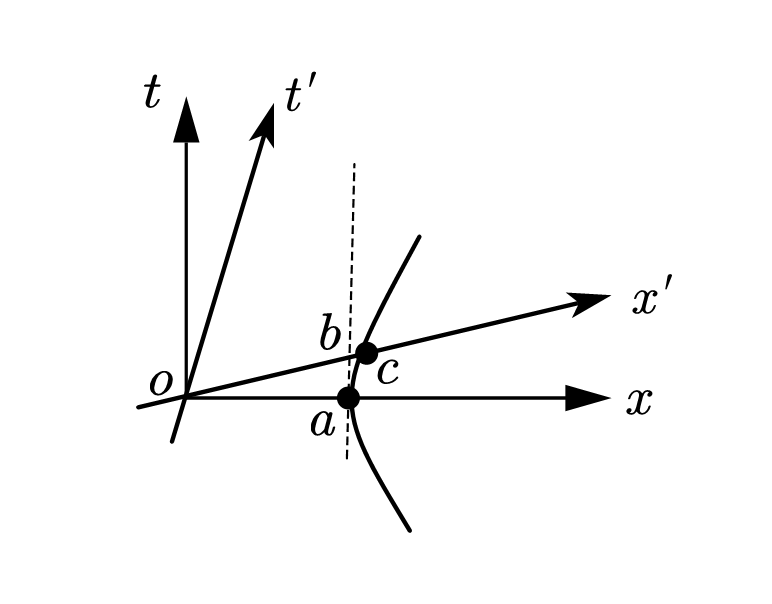
\includegraphics[width=0.8\textwidth]{Pictures/6-8.png}
    \caption{尺缩效应的时空图}
    \label{fig:6-8}
\end{figure}
\subsection{钟慢效应}
\begin{figure}[htbp]
    \centering
    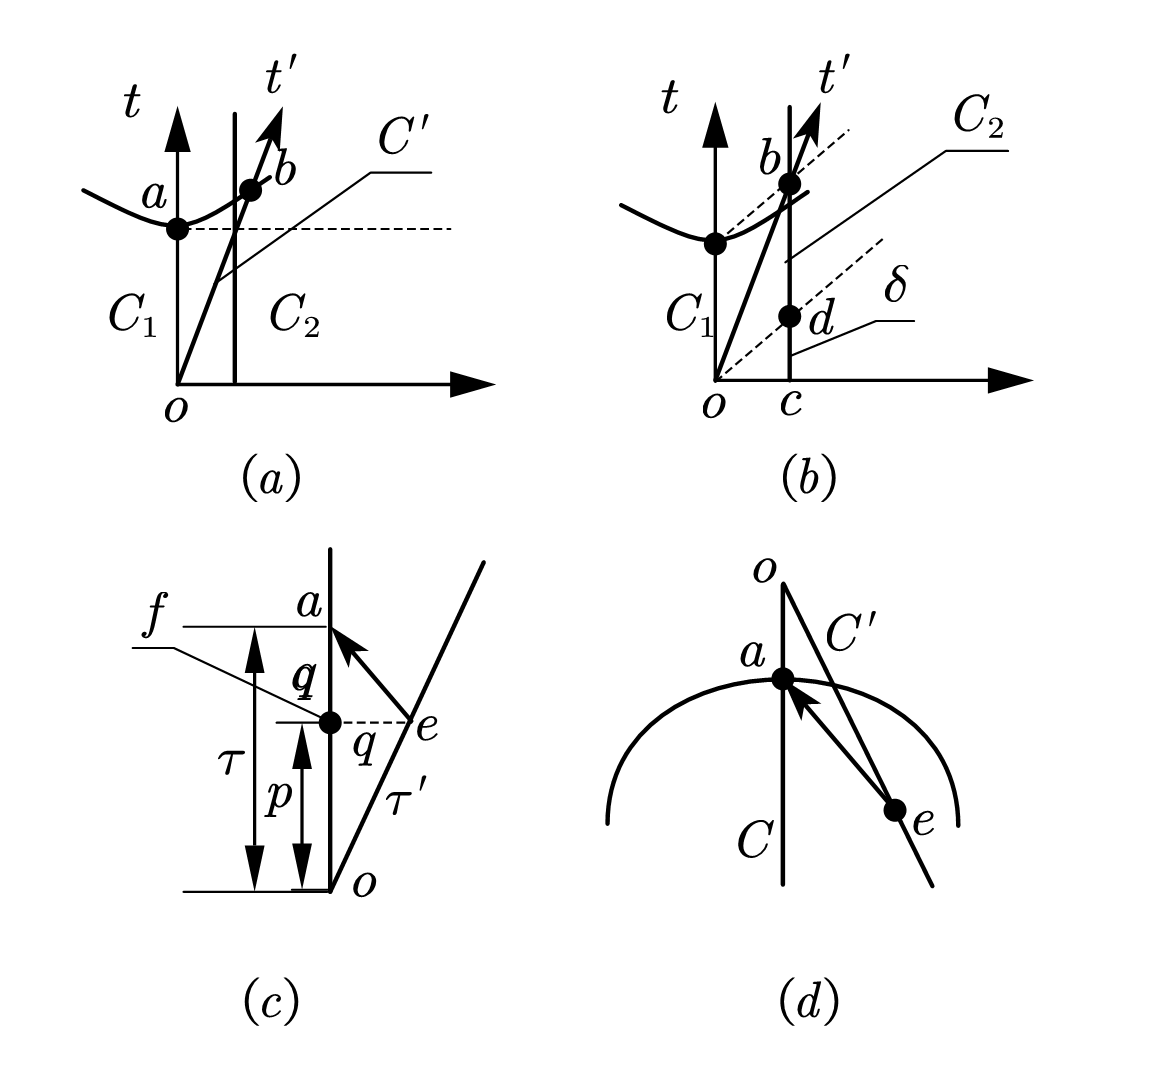
\includegraphics[width=\textwidth]{Pictures/6-9.png}
    \caption{钟慢效应的时空图}
    \label{fig:6-9}
\end{figure}
\subsection{孪子佯谬}
\begin{figure}[htbp]
    \centering
    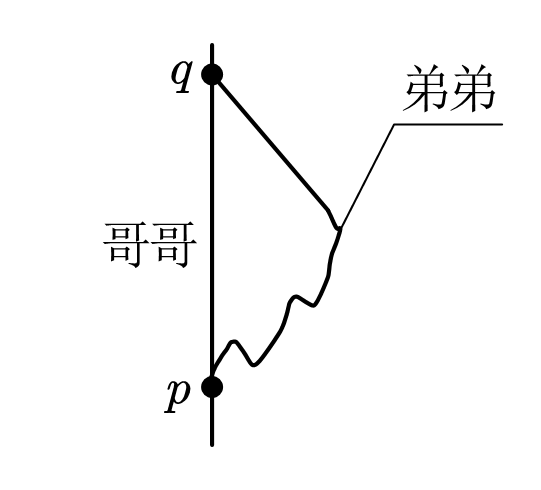
\includegraphics[width=0.6\textwidth]{Pictures/6-10.png}
    \caption{孪子佯谬}
    \label{fig:6-10}
\end{figure}